\chapter{Literature Review}
\label{chap:lit.review}

\section{Introduction}

\subsection{Recurrent Neural Networks}

Recurrent Neural Networks (RNNs) are in forefront of recent development and advances in \textit{deep learning} by making able neural networks to deal with sequences data, which is a major shortcoming in ANN. If the data is based on sequence of events in a video or text, the traditional neural network can't do reasoning for a single event based on its previous one. To tackle this issue RNNs have loops which enables them to persist the information.

\begin{figure}[p]
	\centering
	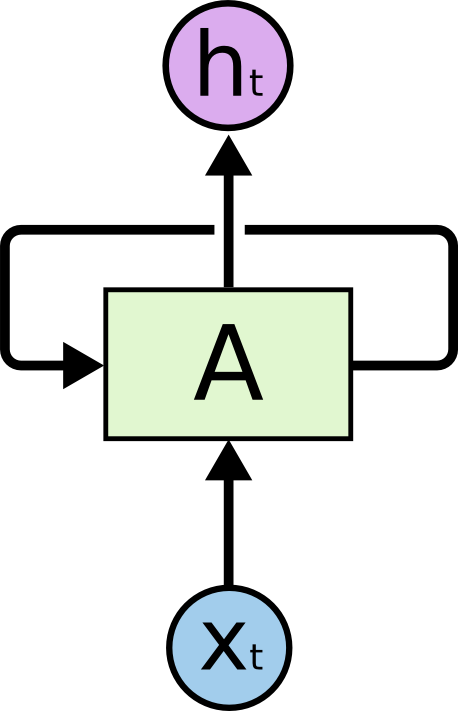
\includegraphics[scale=0.4]{./figs/rnn-rolled}
	\caption[A Rolled Recurrent Neural Networks]{Recurrent Neural Networks (RNNs) uses loops.}
	\label{fig:rnn-rolled}
\end{figure}

As it shown in \textbf{Figure \ref{fig:rnn-rolled}}, a selected neural network, $A$ takes the input $x_t$ and outputs the value of $h_t$. this might not show how data goes from one step to the next one in a same network until you unroll the loop and see chain architecture of recurrent neural networks that makes them the best choice for sequential data, \textbf{Figure \ref{fig:rnn-unrolled}}.

\begin{figure}[p]
	\centering
	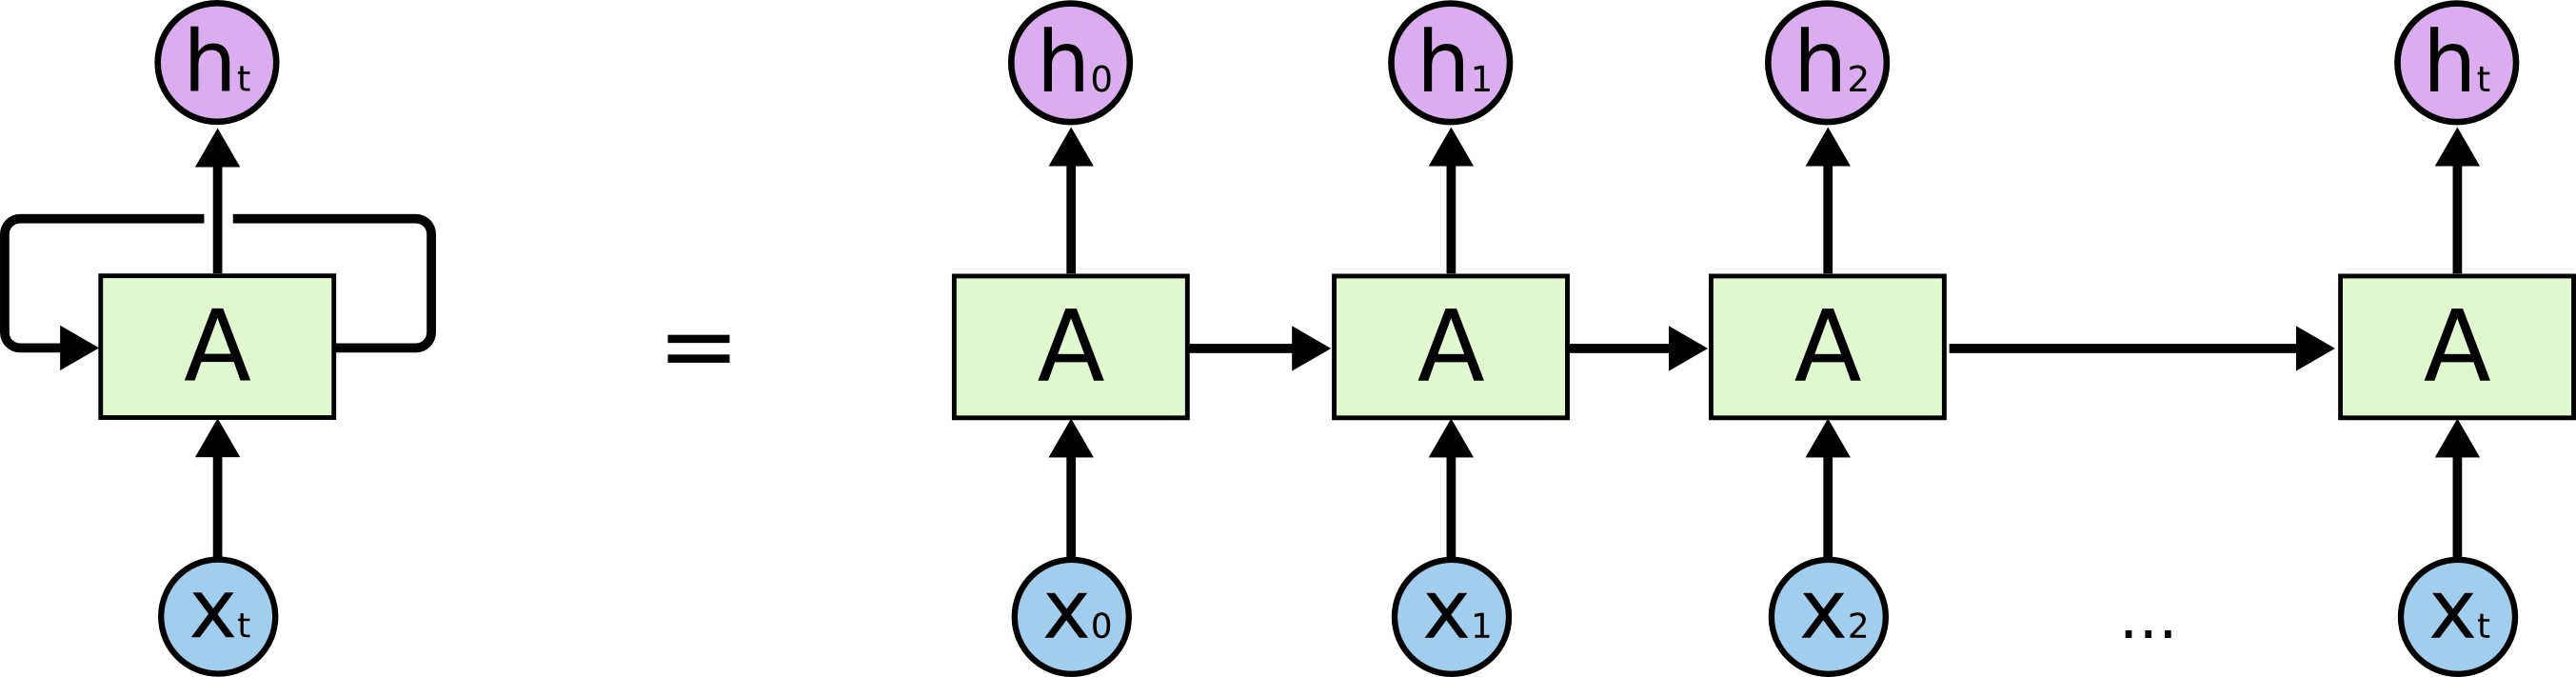
\includegraphics[scale=0.4]{./figs/rnn-unrolled}
	\caption[An Unrolled Recurrent Neural Networks]{An Unrolled Recurrent Neural Networks (RNNs).}
	\label{fig:rnn-unrolled}
\end{figure}

\subsection{Bayes by Backprop}

Bayes by Backprop \cite{Blundell2015a} is a variational inference \cite{Wainwright2008} scheme for learning the posterior distribution on the weights of a neural network.
The posterior distribution on parameters of the network $\theta \in \mathbb{R}^d$, $q(\theta)$ is
typically taken to be a Gaussian with mean parameter $\mu\in \mathbb{R}^d$ and
standard deviation parameter $\sigma\in \mathbb{R}^d$, denoted $\mathcal{N}(\theta|\mu,\sigma)$, noting that we use a diagonal covariance matrix, and where $d$ is the dimensionality of the parameters of the network (typically in the order of millions).
Let $\log p(y|\theta, x)$ be the log-likelihood of the neural network, then the
network is trained by minimising the variational free energy:
\begin{equation}
\label{eq:elbo}
\mathcal{L}(\theta) &=
\mathbb{E}_{q(\theta)}\left[\log \frac{q(\theta)}{p(y|\theta, x)p(\theta)}\right],
\end{equation}
where $p(\theta)$ is a prior on the parameters.

Algorithm~\ref{alg:bbb} shows the Bayes by Backprop Monte Carlo procedure for minimising \ref{eq:elbo} with respect to the mean and standard deviation parameters of the posterior $q(\theta)$.


Minimising the variational free energy \ref{eq:elbo} is equivalent to maximising the log-likelihood $\log p(y|\theta, x)$ subject to a KL complexity term on the parameters of the network that acts as a regulariser:
\begin{equation}
\label{eq:klelbo}
\mathcal{L}(\theta) &=
- \mathbb{E}_{q(\theta)}\left[\log p(y|\theta, x) \right]
+ \kl{q(\theta)}{p(\theta)}.
\end{equation}

In the Gaussian case with a zero mean prior, the KL term can be seen as a form of weight decay on the mean parameters, where the rate of weight decay is automatically tuned by the standard deviation parameters of the prior and posterior.


\begin{algorithm}[ht]
	\caption{Bayes by Backprop}
	\label{alg:bbb}
	\begin{algorithmic}
		\STATE{Sample $\epsilon \sim \mathcal{N}(0, I)$, $\epsilon \in \mathbb{R}^d$.}
		\STATE{Set network parameters to $\theta = \mu + \sigma\epsilon$.}
		\STATE{Do forward propagation and backpropagation as normal.}
		\STATE{Let $g$ be the gradient with respect to $\theta$ from backpropagation.} 
		\STATE{Let $g^{KL}_\theta, g^{KL}_\mu, g^{KL}_\sigma$ be the gradients of $\log \mathcal{N}(\theta|\mu, \sigma) - \log p(\theta)$ with respect to $\theta$, $\mu$ and 
			$\sigma$ respectively.} 
		\STATE{Update $\mu$ according to the gradient $g + g^{KL}_\theta + g^{KL}_\mu$.} 
		\STATE{Update $\sigma$ according to the gradient $(g + g^{KL}_\theta) \epsilon + g^{KL}_\sigma$.}
	\end{algorithmic}
\end{algorithm}

The uncertainty afforded by Bayes by Backprop trained networks has been used successfully for training feedforward models for supervised learning and to aid exploration by reinforcement learning agents \cite{Blundell2015a}, \cite{Lipton2016}, \cite{Houthooft2016}, but as yet, it has not been applied to recurrent neural networks.

\subsection{Model Confidence}

\subsection{Model Uncertainty and Safety}

\section{State-of-the-Arts}

\section{Limitations}
\begin{enumerate}
\item Mentor~Graphics 2
\begin{enumerate}
\item item 3
\end{enumerate}
\item item 4
\end{enumerate}

\section{Research Gaps}
The processing at layer-5%
